% !TeX root = ../main.tex

\section{Approximation of Functions and Data}
    Approximation of data:
    \begin{center}
        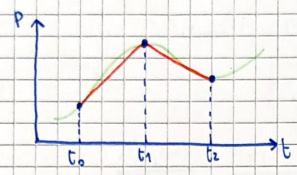
\includegraphics[width=0.5\textwidth]{images/intro_interpolation.png}
        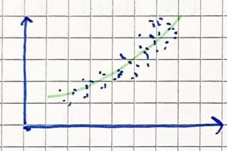
\includegraphics[width=0.45\textwidth]{images/intro_leastsquare.png}
    \end{center}
    Left interpolation, right least square.

    Approximation of functions like integral: approximate it to polynomial. The analytical tool to approximate a function is the Taylor expansion, but it suffers some problems
    \begin{itemize}
        \item Need higher order (more derivatives)
        \item It works well when we consider a neighborhood of the center of the expansion, but moving out of the neighborhood it will start to perform badly
    \end{itemize}

\subsection{Interpolation}
    Instead of Taylor, consider:
    $$
    \begin{bmatrix}
        \text{\textbf{Function}} & & \text{\textbf{Data}}\\
        f & & \Brackets{(x_i,y_i)} \qquad i=0,\cdots,n\\
        y_i=f(x) & & x_i\text{ distinct}
    \end{bmatrix}
    $$
    Identify a function $\tilde{f}$ s.t. $\tilde{f}(x_i)=y_i$ for $i=0,\cdots,n$, \textbf{interpolation conditions}, $n+1$ conditions. The function $\tilde{f}$ can be:
    \begin{itemize}
        \item Polynomial
        \item Trigonometric expansion (Fourier expansion)
        \item Rational
        $$
        \frac{
            a_0+a_1x+\cdots a_px^p
        }{
            b_0+b_1x+\cdots b_qx^q
        }
        $$
    \end{itemize}
    We consider polynomial interpolation

    \subsubsection{Polynomial interpolation}
    \underline{Theorem}: let $\Brackets{x_i,y_i}^n_{i=0}$ ($x_i$ are interpolation nodes, $y_i$ are values to be interpolated) with $x_i$ all distinct. Then $\exists !$ polynomial degree of $\leq n$ (interpolating/interpolation polynomial) s.t. (we guarantee interpolation condition):
    $$
    \underlabel{
        \Pi_n(x_i)=y_i
    }{n+1 conditions}
    \qquad i=0,\cdots,n
    $$
    \underline{Proof for uniqueness}: by contradiction assume that we have 2 interpolating polynomials of order $n$
    $$
    \Pi_n\in\mathbb{P}_n\qquad \Pi_n(x_i)=y_i\qquad i=0,\cdots,n
    $$
    $$
    \Pi_n^*\in\mathbb{P}_n\qquad \Pi_n^*(x_i)=y_i\qquad i=0,\cdots,n
    $$
    Consider the difference
    $$
    D(x)=\Pi_n(x)-\Pi_n^*(x)\in\mathbb{P}_n
    $$
    And
    $$
    D(x_i)=\Pi_n(x_i)-\Pi_n^*(x_i)=y_i-y_i=0\qquad i=0,\cdots,n
    $$
    A polynomial of degree $n$ has at most $n$ intersections with the $x$-axis, but in this case $D(x)$ of degree $n$ has $n+1$ zeros: the only way that we can satisfy the $n+1$ conditions is that $D(x)$ is identically equal to 0. which means
    $$
    D(x)=0\Rightarrow
    \Pi_n(x)-\Pi_n^*(x)=0\Rightarrow
    \Pi_n(x)=\Pi_n^*(x)
    $$
    Which contradicts our initial assumption.

    \underline{Finding the characteristic polynomial}: assume that values to be interpolated are all null except one
    $$
    y_i=0\,\,\forall i\neq k\qquad y_k=1
    $$
    $$
    \begin{Bmatrix}    
        x_0=0 & x_1=0.5 & x_2=1\\
        y_0=0 & y_1=1 & y_2=0
    \end{Bmatrix}
    $$
    Let change notation, instead of $\Pi_2$ we use $\phi_k$
    $$
    \phi_1\in\mathbb{P}_2\qquad
    \underlabel{
        \phi_1(x_0=0)=0
    }{A}\qquad
    \underlabel{
        \phi_1(x_1=1/2)=1
    }{B}\qquad
    \underlabel{
        \phi_1(x_2=1)=0
    }{C}\qquad
    $$
    We want to build a polynomial of degree 2 that is zero in those two points:
    $$
    \begin{cases}
        (x-0)(x-1)\qquad\text{satisfies A and B}\\
        \frac{
            (x-0)(x-1)
        }{
            (0.5-0)(0.5-1)
        }\qquad\text{satisfies C}
    \end{cases}
    $$
    $$
    \phi_1(x)=\cdots=-4x(x-1)
    $$
    With a generic case
    $$
    \phi_k(x_i)=\delta_{ik}=\begin{cases}
        0\qquad i\neq k\\
        1\qquad i=k
    \end{cases}
    $$
    Kronecker delta, to express it as a polynomial with degree $n$, the characteristic polynomial:
    \begin{LARGE}
        $$
        \phi_k(x)=
        \prod_{j=0,j\neq k}^n
        \frac{
            x-x_j
        }{
            x_k-x_j
        }
        $$
    \end{LARGE}
    \underline{Moving to a more general case}: instead of a set of arbitrary values
    $$
    \begin{Bmatrix}
        x_0 & x_1 & x_2\\
        y_0 & y_1 & y_2\\
        \Pi(x_0)=y_0 & \Pi(x_1)=y_1 & \Pi(x_2)=y_2
    \end{Bmatrix}
    $$
    Expressing $\Pi_2$ as linear combination of $\phi_0$, $\phi_1$ and $\phi_2$
    $$
    \begin{Bmatrix}
        \phi_0 & \phi_0(x_0)=1 & \phi_0(x_1)=0 & \phi_0(x_2)=0\\
        \phi_1 & \phi_1(x_0)=0 & \phi_1(x_1)=1 & \phi_1(x_2)=0\\
        \phi_2 & \phi_2(x_0)=0 & \phi_2(x_1)=0 & \phi_2(x_2)=1
    \end{Bmatrix}
    $$
    $$
    \Pi_2(x)=a\phi_0(x)+b\phi_1(x)+c\phi_2(x)
    $$
    Solving we will get:
    $$
    a=y_0\qquad b=y_1\qquad c=y_2
    $$
    The \textbf{Lagrange form}:
    \begin{LARGE}
        $$
        \Pi_n(x)=\sum_{k=0}^ny_k\phi_k(x)
        $$
        $$
        \Pi_n(x)=\sum_{k=0}^ny_k\prod_{j=0,j\neq k}^n
        \frac{
            x-x_j
        }{
            x_k-x_j
        }
        $$
    \end{LARGE}
    In matlab:
    \begin{itemize}
        \item \textbf{c = polyfit(x,y,n)}, to build interpolating polynomial
        \begin{itemize}
            \item x vector collecting interpolation nodes, $x_i$
            \item y is $y_i$
            \item n is the degree of the polynomial, but is redundant as there is a strict relation between number of data and degree of polynomial (for $n$ data, the polynomial will have defree of $n-1$), in least squares it will have a meaning
        \end{itemize}
        It returns the coefficients of our interpolating polynomial
        $$
        p_n(x)=a_nx^n+a_{n-1}x^{n-1}+\cdots+a_1x+a_0
        $$
        With c(1) coefficient of $x^n$, c(2) of $x(n-1)$
        \item \textbf{d = polyval(c,z)}, to evaluate interpolating polynomial at point $z$
        \begin{itemize}
            \item If z single number $\mathbb{R}$, d will be a number
            \item If z is $\mathbb{R}^q$, vector
        \end{itemize}
    \end{itemize}

    \subsubsection{Interpolation error}
    Error at nodes is null, at points that are not nodes? Consider a function continuous in a certain interval $I$:
    $$
    f\in C^0(\overline{I})\qquad I (x_0,x_n)
    $$
    $$
    \Brackets{(x_i,y_i=f(x_i))}^n_{i=0}\qquad x_i\text{ distinct}
    $$
    Assuming
    $$
    f\in C^{n+1}(\overline{I})
    $$
    We define the interpolation error:
    $$
    \forall\,\,x\in\,\,I
    $$
    $$
    E_nf(x)=f(x)-\Pi_nf(x)=\frac{
        f^{(n+1)}\left(\alpha(x)\right)
    }{
        (n+1)!
    }\prod_{k=0}^n (x-x_k)
    $$
    And as expected $E_nf(x_i)=0$. The weak point is that we assume regularity in the function, which depends on the number of nodes: such regularity uncommon. Another drawback is that the $\alpha(x)$ depends on $x$ but we don't know the exact value of $\alpha(x)\in I$. In practice this result useless, so we consider the maximum value.

    If we have more and more information, more samples, the degree of polynomial increases and we have more zeros (the function meets the x axis more times, like sinusoid) but the quality of the approximation improves.\\
    Consider an uniform partition of the interval
    \begin{center}
        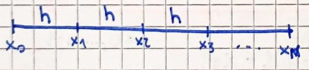
\includegraphics[width=0.7\textwidth]{images/uniform_dist.png}
    \end{center}
    $$
    h=\frac{x_n-x_0}{n}
    $$
    $$
    x_k=x_{k+1}+h\qquad k=1,\cdots,n
    $$
    $$
    x_j=x_0+jh\qquad j=0,\cdots,n
    $$
    In this case we can prove:
    $$
    \left|
        \prod_{k=0}^n(x-x_k)
    \right|\leq
    n!\frac{h^{n+1}}{4}
    $$
    Therefore:
    \begin{LARGE} 
    $$
    \max_{x\in I}\left|E_nf(x)\right|
    \leq
    \underlabel{
        \frac{
            h^{n+1}
        }{
            4(n+1)
        }
    }{A}
    \cdot
    \underlabel{
        \max_{x\in I}\left|
            f^{(n+1)}(x)
        \right|
    }{B}
    $$
    \end{LARGE}
    The two blocks:
    \begin{itemize}
        \item A$\rightarrow$0 for $n\rightarrow\infty$
        \item B for $n\rightarrow\infty$ depends on $f$:
        $$
        \text{B}\rightarrow
        \begin{cases}
            0\\
            \text{constant}\\
            +\infty\begin{cases}
                \text{If A goes to 0 quicker, OK}\\
                \text{If B goes to $\infty$ quicker, not OK}
            \end{cases}
        \end{cases}
        $$
    \end{itemize}
    Consider infact the function
    $$
    f(x)=\frac{1}{1+x^2}\qquad x\in I =\left[-5,5\right]
    $$
    \begin{center}
        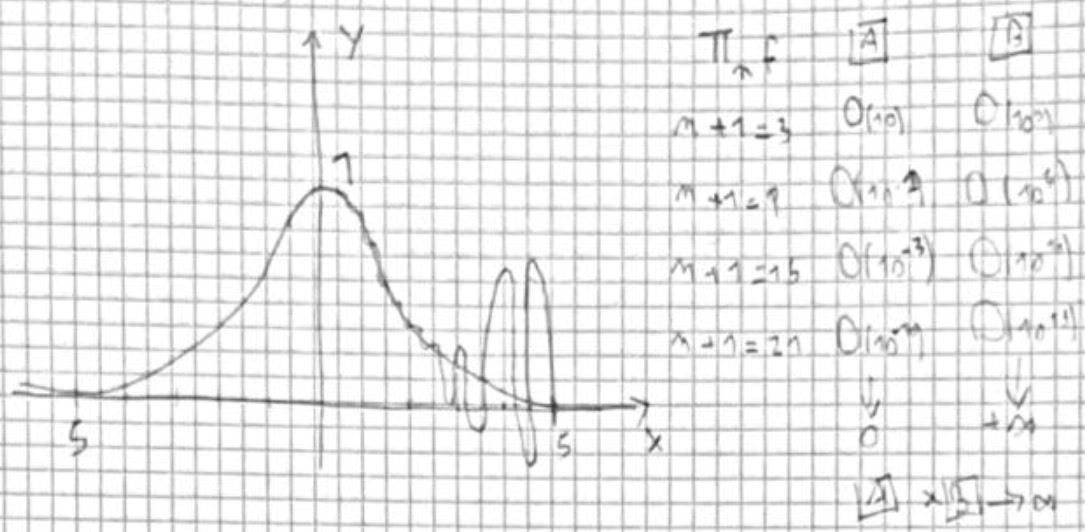
\includegraphics[width=0.9\textwidth]{images/runge.png}
    \end{center}
    We are in presence of spurious oscillations, in the case this error goes to $\infty$, we have the \textbf{Runge phenomenon: more samples, possibility of spurious oscillations}.\\
    To deal with this we can:
    \begin{itemize}
        \item Particular choice of nodes, Chebyshev nodes, as we chose uniform sampling, uniform distribution of nodes, not good idea: with Chebyshev we choose more nodes near the endpoints where the Runge phenomenon occurs, while at the center of the interval less nodes. To divide into $n$ parts:
        \begin{enumerate}
            \item $n$ equal parts first
            $$
            \frac{\Pi_i}{n}\qquad i=0,\cdots,n
            $$
            \item Compute the projection on the x-axis, the minus sign is in order to fix the order
            $$
            -f\left(
                \frac{\Pi_i}{n} 
            \right)
            $$
            \item To use Chebyshev, use the following function that maps the interval $I$ to the generic interval $[a,b]$, maps the nodes of previous step
            $$
            x_i=\frac{a+b}{2}+\frac{b-a}{2}\hat{x}_i
            $$
        \end{enumerate}
        \item When we increase $n$, a lot of x-axis crosses, so we can use low degree polynomials and work interval by interval: \textbf{piecewise linear interpolation}
    \end{itemize}
    
    \subsubsection{Piecewise linear interpolation}
    We do not have to select an uniform distribution of nodes
    $$
    I_j=\left[x_j,x_{j+1}\right]\qquad h_j=x_{j+1}-x_j
    $$
    $$
    H=\max_jh_j
    $$
    The idea is consider each subinterval and replace the function $f$ with conjuction of endpoints (polynomial with low degree, so we avoid oscillations). By increasing the number of nodes, the approximation improves
    \begin{center}
        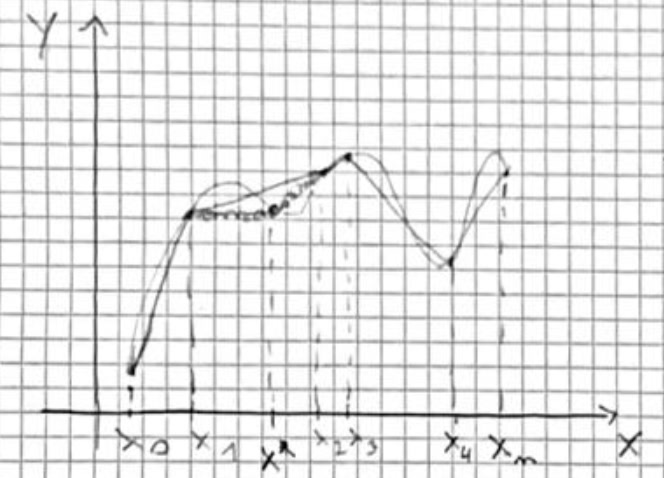
\includegraphics[width=0.7\textwidth]{images/piecewise.png}
    \end{center}
    We indicate linear interpolant as:
    $$
    \Pi_1^Hf\in C^0(\overline{I})
    $$
    $$
    \Pi_1^Hf\Big|_{I_j}\in \mathbb{P}_1(I_j)
    $$
    $$
    \Pi_i^Hf(x_k)=f(x_k)\qquad k=0,\cdots,n
    $$
    Express it as conjuction of endpoints that includes those 3 requirements:
    \begin{LARGE}
        $$
        \Pi_1^Hf(x)=f(x_j)+\frac{
            f(x_{j+1})-f(x_j)
        }{
            x_{j+1}-x_j
        }(x-x_j)\qquad
        x\in I_j
        $$
    \end{LARGE}
    How to prove that the error becomes 0 for $n\rightarrow\infty$? We consider the local error on the subintervals $I_j$, we have (for $n=1$):
    \begin{LARGE}
        $$
        \max_{x\in I_j}\left|E_1^Hf(x)\right|
        \leq
        \frac{
            h_j^2
        }{
            4\cdot(1+1)
        }\cdot
        \max_{x\in I_j}\left|
            f''(x)
        \right|\qquad
        f\in C^2(\overline{I}_j)
        $$
    \end{LARGE}
    Instead of $I_j$ and $h_j$, we want inequality on all $I$:
    \begin{LARGE}
        $$
        \max_{x\in I}\left|E_1^Hf(x)\right|
        \leq
        \frac{
            H^2
        }{
            8
        }\cdot
        \max_{x\in I}\left|
            f''(x)
        \right|\qquad
        f\in C^2(\overline{I})
        $$
    \end{LARGE}
    Now we have the error that is decreasing:
    \begin{itemize}
        \item A = $\frac{H^2}{8}$, for $n\rightarrow\infty$, the maximum length $H$ will become smaller and smaller as we are increasing samples!
        \item B = $\max_{x\in I}\left|f''(x)\right|$ does not change, it's not dependent on $n$
    \end{itemize}
    We can also use piecewise parabola or cubic interpolation, when we join pieces of parabola is the approximation more regular? Is it a $C^1$ or still $C^0$? Not $C^1$, so by increasing local degree of polynomial we do not gain regularity, but we are improving accuracy of approximation. For example $n=2$
    $$
        \max_{x\in I_j}\left|E_2^Hf(x)\right|
        \leq
        \frac{
            h_j^3
        }{
            4\cdot(2+1)
        }\cdot
        \max_{x\in I_j}\left|
            f^{(3)}(x)
        \right|\qquad
        f\in C^3(\overline{I}_j)
    $$
    $$
    \max_{x\in I}\left|E_1^Hf(x)\right|
    \leq
    \frac{
        H^3
    }{
        12
    }\cdot
    \max_{x\in I}\left|
        f^{(3)}(x)
    \right|\qquad
    f\in C^3(\overline{I})
    $$
    This is a problem, we would like something that is globally very smooth.

    In matlab:
    \begin{itemize}
        \item \textbf{d = interp1(x,y,z)}, in some sense merges both polyfit and polyval, output will have same dimension as z
        \item \textbf{d = interp2(x,y,z)}, cubic interpolation
    \end{itemize}
    A remark: the matlab function plot is doing a sampling of the function, which is finer in the gradient of the function. This is known as \textbf{adaptive sampling}

    \subsubsection{Cubic spline interpolation}
    Again, a piecewise interpolation, but we join endpoints with a cubic function
    \begin{enumerate}
        \item $S_3\Big|_{I_j}\in\mathbb{P}$
        \item Spline means function \textbf{smooth globally}, the pieces are joined so that the function is globally, $S_3\in C^2(\overline{I})$
        \item $S_3(x_i)=f(x_i)\qquad i=0,\cdots,n$
    \end{enumerate}
    In matlab \textbf{d = spline(x,y,z)}, build and directly evaluate. For each interval we have a polynomial of degree 3: $S_3$ (so $a_i$ for $i=4$).We have 4 unknowns for each interval, let \#intervals = $n$, so $4n$ unknowns. The procedure:
    \begin{enumerate}[1)]
        \item $S_3((x_i)=f(x_i)\qquad i=0,\cdots,n$
        \item We demand $S_3$ continuous in the nodes, $S_3\in C^0\left(\left[
            x_0,x_n
        \right]\right)$
        $$
        \left[S_3(x_i)\right]^-=
        \left[S_3(x_i)\right]^+
        \qquad i=1,\cdots,n-1
        $$
        \item We demand $S_3'$ continuous in the nodes, $S_3'\in C^0\left(\left[
            x_0,x_n
        \right]\right)$
        $$
        \left[S_3'(x_i)\right]^-=
        \left[S_3'(x_i)\right]^+
        \qquad i=1,\cdots,n-1
        $$
        \item We demand $S_3''$ continuous in the nodes, $S_3''\in C^0\left(\left[
            x_0,x_n
        \right]\right)$
        $$
        \left[S_3''(x_i)\right]^-=
        \left[S_3''(x_i)\right]^+
        \qquad i=1,\cdots,n-1
        $$
    \end{enumerate}
    In total we have $(n+1)+3(n-1)=4n-2$ conditions, but we need two more:
    \begin{itemize}
        \item $S_3''(x_0)=S_3''(x_n)=0$, natural cubic interpolating spline
        \item Not-a-knot-condition: $S_3''$ continuous at $x_1,x_{n-1}$
        $$
        \left[
            S_3'''(x_1)
        \right]^-=
        \left[
            S_3'''(x_1)
        \right]^+
        \qquad
        \left[
            S_3'''(x_{n-1})
        \right]^-=
        \left[
            S_3'''(x_{n-1})
        \right]^+
        $$
    \end{itemize}
    The error:
    $$
    \max_{x\in\left[x_0,x_n\right]}
    \left|
        f^{(r)}(x)-
        S_3^{(r)}(x)
    \right|\leq
    C_r\cdot
    H^{4-r}\cdot
    \max_{x\in\left[x_0,x_n\right]}
    \left|
        f^{(4)}(x)
    \right|
    \qquad r=0,1,2
    $$

\subsection{Least Squared Approximation}
    Data $\Brackets{(x_i,y_i)}^n_{i}$, $x_i$ distinct, we find a polynomial $\tilde{f}\in\mathbb{P}_m$ of degree $m\geq 1,m<<n$ and $\tilde{f}(x_i)\neq y_i$ such that:
    \begin{LARGE}
        $$
        \underlabel{
            \sum_{i=0}^m\left[\tilde{f}(x_i)-y_i\right]^2
        }{A}
        \leq
        \underlabel{
            \sum_{i=0}^n\left[p_m(x_i)-y_i\right]^2
        }{B}
        \qquad\forall\,\,p_m\in\mathbb{P}_m
        $$
    \end{LARGE}
    We want to minimize the right term.
    \subsubsection{Degree n}
    $m=n$ Lagrange interpolant, $\tilde{f}==\Pi_n$

    \subsubsection{Degree 1}
    $m=1$ regression line
    $$
    p_1(x)=b_0+b_1x\qquad b_0,b_1\in\mathbb{R}
    $$
    $$
    \tilde{f}(x)=a_0+a_1x\qquad a_0,a_1\in\mathbb{R}
    $$
    We want to find the specific polynomial $\tilde{f}$ (so the two coefficients). Consider the definition, the blocks:
    \begin{itemize}
        \item A = $\sum_{i=0}^n\left[a_0+a_1x_i-y_i\right]^2=\Phi(a_0,a_1)$
        \item B = $\sum_{i=0}^n\left[b_0+b_1x_i-y_i\right]^2=\Phi(b_0,b_1)$
    \end{itemize}
    So:
    $$
    \Phi(a_0,a_1)\leq\Phi(b_0,b_1)\qquad\forall\,\,b_0,b_1\in\mathbb{R}
    $$
    We compute the partial derivatives to find $a_0$ and $a_1$:
    $$
    \frac{
        \partial\Phi
    }{\partial b_0}\Big|_{(b_0,b_1)=(a_0,a_1)}=0
    \qquad
    \frac{
        \partial\Phi
    }{\partial b_1}\Big|_{(b_0,b_1)=(a_0,a_1)}=0
    $$
    By developing $\Phi(b_0,b_1)$
    $$
    \Phi(b_0,b_1)=
    \sum_{i=0}^n\left[b_0^2+b_1^2x_i^2+y_i^2+2b_0b_1x_i-2b_0y_i-2b_1x_iy_i\right]
    $$
    And the partial derivatives:
    $$
    \frac{
        \partial\Phi
    }{\partial b_0}=\sum_{i=0}^n\left[
        2b_0+2b_1x_i-2y_i
    \right]
    \qquad
    \frac{
        \partial\Phi
    }{\partial b_0}=\sum_{i=0}^n\left[
        2b_1x_i^2+2b_0x_i-2x_iy_i
    \right]
    $$
    Putting $a_0$ and $a_1$
    $$
    \begin{cases}            
        \sum_{i=0}^n\left[
            2a_0+2a_1x_i-2y_i
        \right]=0
        \\
        \sum_{i=0}^n\left[
            2a_1x_i^2+2a_0x_i-2x_iy_i
        \right]=0
    \end{cases}\rightarrow B\overrightarrow{a}=\overrightarrow{f}
    $$
    $$
    \begin{cases}            
        \sum_{i=0}^na_0+\sum_{i=0}^na_1x_i=\sum_{i=0}^ny_i
        \\
        \sum_{i=0}^na_1x_i^2+\sum_{i=0}^na_0x_i=\sum_{i=0}^nx_iy_i
    \end{cases}
    \Rightarrow
    \begin{cases}            
        a_0(n+1)+a_1\sum_{i=0}^nx_i=\sum_{i=0}^ny_i
        \\
        a_1\sum_{i=0}^nx_i^2+a_0\sum_{i=0}^nx_i=\sum_{i=0}^nx_iy_i
    \end{cases}
    $$
    $$
    B=\begin{bmatrix}
        (n+1) & \sum x_i\\
        \sum x_i & \sum x_i^2
    \end{bmatrix}\qquad
    \overrightarrow{f}=\left[
        \sum y_i,\sum x_iy_i
    \right]^T\qquad
    \overrightarrow{a}=\left[
        a_0,a_1
    \right]^T
    $$
    Where $B$ is spd (we can use gradient method)

    \subsubsection{Degree m generic}
    $$
    \tilde{f}(x)=a_0+a_1x+a_2x^2+\cdots+a_mx^m
    $$
    $$
    p_m(x)=b_0+b_1x+b_2x^2+\cdots+b_mx^m
    $$
    $$
    \frac{
        \partial\Phi
    }{b_i}\Big|_{(b_0,b_1,\cdots,b_m)=(a_0,a_1,\cdots,a_m)}=0\qquad i=0,\cdots,m
    $$
    Just like before, we wanto to find $a_0,\cdots,a_m$, after the calculations:
    $$
    B=\begin{bmatrix}
        (n+1) & \sum x_i & \sum x_i^2 & \cdots & \sum x_i^m\\
        \sum x_i & \sum x_i^2 & \sum x_i^3 & \cdots & \sum x_i^{m+1}\\
        \vdots\\
        \sum x_i^m & \sum x_i^{m+1} & \sum x_i^{m+2} & \cdots & \sum x_i^{2m}
    \end{bmatrix}
    $$
    $$
    \overrightarrow{a}=\begin{bmatrix}
        a_0\\
        a_1\\
        \vdots\\
        a_m
    \end{bmatrix}\qquad
    \overrightarrow{f}=\begin{bmatrix}
        \sum y_i\\
        \sum x_iy_i\\
        \vdots\\
        x_i^my_i
    \end{bmatrix}
    $$

\subsection{Numerical Integration}
$$
I(f)=\int_{a}^bf(x)dx\qquad
f\in C^0\left([a,b]\right)
$$
The quadrature rule: approximate a function:
$$
\tilde{I}(f)\simeq I(f)
$$
$$
\tilde{I}(f)=\int_{a}^b\tilde{f}(x)dx\qquad
\tilde{f}(x)\simeq f(x)
$$
The steps:
\begin{itemize}
    \item Subdivide into $M$ intervals, the points are known as quadrature nodes
    \begin{center}
        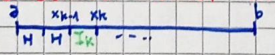
\includegraphics[width=0.5\textwidth]{images/quadrature_nodes.png}
    \end{center}
    $M+1$ points, so $M$ intervals, $x_i$ are quadrature nodes. The amplitude:
    $$
    H=\frac{b-a}{M}
    $$
    Uniform partition of quadrature nodes:
    $$
    x_{i+1}=x_i+H\qquad
    i=0,\cdots,M-1
    $$
    $$
    x_i=x_0+(i)H\qquad i=1,\cdots,M
    $$
    \item Expand the additivity and associativity of integral:
    \begin{LARGE}
        $$
        \int_{a}^bf(x)dx=\sum_{k=1}^M\int_{I_k}f(x)dx\cong
        \sum_{k=1}^M\int_{I_k}\tilde{f}(x)dx=\tilde{I}(f)
        $$
    \end{LARGE}
    With $\tilde{f}(x)\in\mathbb{P}_m$, for different choices of $m$ different quadrature rules
\end{itemize}

\subsubsection{Newton-Cotes}
Interpolatory quadrature rule:
\begin{LARGE}
    $$
    \tilde{I}(f)=\sum_{i=1}^J\alpha_if(x_i)
    $$
\end{LARGE}
With $\alpha_i$ quadrature weights, $x_i$ quadrature nodes. We have first to define:
\begin{itemize}
    \item \textbf{Order of accuracy}, associated only to the composite rule, "rate of convergence for the quadrature rule to zero- of the error" (it's the power of $H$ in the composite error): \textbf{it's the convergence rate, that we can compute with piecewise by plotting $H$ against the error, $H$, $H^2$, till $n$ of $C^n$ in loglog and take the line parallel to the error}
    \item \textbf{Degree of exactness}, associated both to composite and simple, maximum degree of the polynomials which are exactly integrated by your quadrature rule. Suppose:
    $$
    I(f)=\int_a^bf(x)dx\qquad\tilde{I}(f)
    $$
    We start from polynomial of degree 0 $p_0$, but they are infinite: choose a representant
    $$
    I(1)=?=\tilde{I}(1)
    $$
    Then continue till this check does not hold. But in practice the following equality holds:
    $$
    de=\text{[degree of derivative]}-1
    $$
    If we know the explicit expression of the error ($E$) we try different degrees in order to make it zero: $de$ is the order of derivative-1
\end{itemize}
We have
\begin{itemize}
    \item $m=0$, \textbf{midpoint quadrature rule}, which means for each subinterval $\tilde{f}$ is a constant function
    \begin{center}
        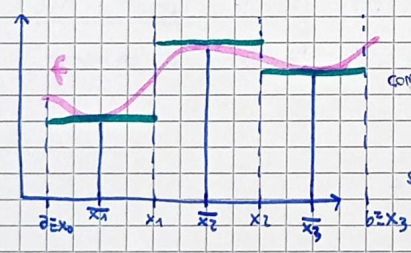
\includegraphics[width=0.5\textwidth]{images/quadrature_m0.png}
    \end{center}
    $$
    \begin{cases}
        \tilde{f}\in\mathbb{P}_0\\
        I_k=[x_{k-1},x_k]\\        
        \overline{x}_k=\frac{x_{k-1}+x_k}{2}
    \end{cases}
    $$
    The composite midpoint quadrature rule:
    \begin{LARGE}
        $$
        \tilde{I}_{MP}^c(f)=H\sum_{k=1}^Mf(\overline{x}_k)
        $$
    \end{LARGE}
    Where $c$ stands for composite, the simple midpoint quadrature rule version:
    \begin{LARGE}
        $$
        \tilde{I}_{MP}(f)=(b-a)f\left(\frac{a+b}{2}\right)
        $$
    \end{LARGE}
    \textbf{Errors}:
    \begin{itemize}
        \item Simple midpoint quadrature rule error
        $$
        I(f)-\tilde{I}_{MP}(f)=\int_a^b\left[f(x)-f(\overline{x})\right]
        $$
        Use the Taylor expansion centered at $\overline{x}$, $f\in C^2([a,b])$, second order:
        $$
        f(x)-f(\overline{x})=f'(\overline{x})(x-\overline{x})+
        \frac{f''(\alpha(x))}{2}(x-\overline{x})^2
        $$
        Making the computations...
        $$
        \tilde{E}_{MP}=I(f)-\tilde{I}_{MP}(f)=
        \frac{(b-a)^3}{24}f''(\beta)
        $$
        $$
        f\in C^2([a,b])\qquad\beta\in[a,b]
        $$
        $\beta$ (from min value theorem of integral) cannot be found, in practice upperbound for worst case
        \item Composite midpoint quadrature rule error
        $$
        I(f)-\tilde{I}_{MP}^c(f)=\sum_{k=1}^M\left[
            \int_{I_k}f(x)dx-
            \tilde{I}_{MP}\left(f\big|_{I_k}\right)
        \right]=
        \sum_{k=1}^M\frac{H^3}{24}f''(\beta_k)
        $$
        Again from min value theorem of summation (dual of integral one):
        $$
        =\frac{H^3}{24}f''(\gamma)\sum_{k=1}^M1=
        =\frac{H^3}{24}f''(\gamma)M=
        $$
        With $H=\frac{b-a}{M}\rightarrow M=\frac{b-a}{M}$, so:
        $$
        \tilde{E}_{MP}^c=I(f)-\tilde{I}_{MP}^c(f)=
        \frac{(b-a)}{24}H^2f''(\gamma)
        $$
        $$
        f\in C^2([a,b])\qquad\gamma\in[a,b]
        $$
    \end{itemize}
    \textbf{Order of accuracy}: $oa_{MP}=2$\\
    \textbf{Degree of exactness}: $de_{MP}=1$
    \begin{itemize}
        \item $p_0$ degree 0
        $$I(1)=?=\tilde{I}(1)$$
        $$
        (b-a)=?=(b-a)f\left(\frac{a+b}{2}\right)=(b-a)
        $$
        OK
        \item $p_1$ degree 1
        $$I(x)=?=\tilde{I}(x)$$
        $$
        \frac{x^2}{2}\Big|_a^b=?=(b-a)\frac{a+b}{2}
        $$
        OK, make the computations
        \item $p_2$ degree 2
        $$I(x^2)=?=\tilde{I}(x^2)$$
        $$
        \frac{x^3}{3}\Big|_a^b=?=(b-a)\left[\frac{a+b}{2}^2\right]
        $$
        KO, we stop here, so $de_{MP}=1$
    \end{itemize}

    \item $m=1$, \textbf{trapezoidal quadrature rule}, for each subinterval a linear function
    \begin{center}
        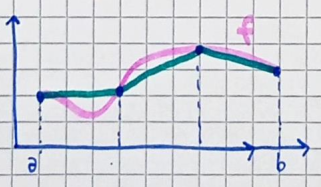
\includegraphics[width=0.5\textwidth]{images/quadrature_m1.png}
    \end{center}
    The composite trapezoidal quadrature rule (just basis times height):
    \begin{LARGE}
        $$
        \tilde{I}_{T}^c(f)=
        \frac{H}{2}
        \sum_{k=1}^M
        \left[
            f(x_{k-1})+f(x_k)
        \right]=
        \frac{H}{2}
        \left[
            f(a)+f(b)
        \right]+
        H\sum_{k=1}^{M-1}f(x_k)
        $$
    \end{LARGE}
    The first expression associated to intervals, the second to nodes. The simple trapezoidal quadrature rule version:
    \begin{LARGE}
        $$
        \tilde{I}_T(f)=\frac{(b-a)}{2}\left[f(a)+f(b)\right]
        $$
    \end{LARGE}
    \textbf{Errors}:
    \begin{itemize}
        \item Simple trapezoidal quadrature rule
        $$
        I(f)-\tilde{I}_T(f)=\int_a^b\left[d(x)-\Pi_1(f)(x)\right]dx
        $$
        The term inside the integral is:
        $$
        E_1=\frac{f''(\eta(x))}{2}(x-a)(a-b)
        $$
        From
        $$
        E_nf(x)=\frac{f^{(n+1)}(\alpha(x))}{(n-1)!}\prod_{k=0}^n(x-x_k)
        $$
        Making the computations...
        $$
        \tilde{E}_T=I(f)-\tilde{I}_T(f)=
        -\frac{(b-a)^3}{12}f''(\delta)
        $$
        $$
        f\in C^2([a,b])\qquad\delta\in[a,b]
        $$
        \item Composite trapezoidal quadrature rule
        $$
        \tilde{E}_T^c=I(f)-\tilde{I}_T^c(f)=
        -\frac{(b-a)}{12}H^2f''(\rho)
        $$
        $$
        f\in C^2([a,b])\qquad\rho\in[a,b]
        $$
    \end{itemize}
    \textbf{Order of accuracy}: $oa_{T}=2$\\
    \textbf{Degree of exactness}: $de_{T}=1$\\
    Though $oa$ and $de$ same as midpoint, we see that the error is twice that of the midpoint: midpoint is easier and has lower error
    \item $m=2$, \textbf{Simpson quadrature rule}
    \begin{center}
        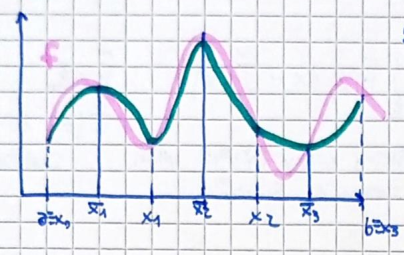
\includegraphics[width=0.5\textwidth]{images/quadrature_m2.png}
    \end{center}
    \begin{LARGE}
        $$
        \tilde{I}_{S}^c(f)=
        \frac{H}{6}
        \sum_{k=1}^M
        \left[
            f(x_{k-1})+4f(\overline{x}_k)+f(x_k)
        \right]=
        $$
        $$
        =
        \frac{H}{6}
        \left[f(a)+f(b)\right]+
        \frac{H}{3}
        \sum_{k=1}^{M-1}f(x_k)+
        \frac{2}{3}H
        \sum_{k=1}^{M}f(\overline{x}_k)
        $$
    \end{LARGE}
    The simple Simpson quadrature rule version:
    \begin{LARGE}
        $$
        \tilde{I}_S(f)=\frac{(b-a)}{6}\left[
            f(a)+
            4f\left(\frac{a+b}{2}\right)+f(b)
        \right]
        $$
    \end{LARGE}
    \textbf{Errors}:
    \begin{itemize}
        \item Simple Simpson quadrature rule
        $$
        \tilde{E}_S=I(f)-\tilde{I}_S(f)=
        -\frac{(b-a)^5}{2880}f^{(4)}(\sigma)
        $$
        $$
        f\in C^4([a,b])\qquad\sigma\in[a,b]
        $$
        \item Composite Simpson quadrature rule
        $$
        \tilde{E}_S^c=I(f)-\tilde{I}_S^c(f)=
        -\frac{(b-a)}{2880}H^4f^{(4)}(\eta)
        $$
        $$
        f\in C^4([a,b])\qquad\eta\in[a,b]
        $$
    \end{itemize}
    \textbf{Order of accuracy}: $oa_{S}=4$\\
    \textbf{Degree of exactness}: $de_{S}=3$
    \begin{itemize}
        \item $p_0$ degree 0
        $$I(1)=?=\tilde{I}(1)$$
        $$
        (b-a)=?=
        \frac{(b-a)}{6}\left[
            f(a)+
            4f\left(\frac{a+b}{2}\right)+f(b)
        \right]=
        \frac{(b-a)}{6}\left[
            1+
            4+1
        \right]
        =(b-a)
        $$
        As $f$ is 1 evaluated everywhere.\\
        OK
        \item $p_1$ degree 1
        $$I(x)=?=\tilde{I}(x)$$
        $$
        \frac{x^2}{2}\Big|_a^b=?=
        \frac{(b-a)}{6}\left[
            f(a)+
            4f\left(\frac{a+b}{2}\right)+f(b)
        \right]
        $$
        OK, make the computations
        \item $p_2$ degree 2\\
        OK
        \item $p_3$ degree 3\\
        KO, we stop here, so $de_{S}=3$
    \end{itemize}
\end{itemize}

\subsubsection{Gaussian quadrature rules}
Till now we have seen Newton-Cotes formulas, while now we will see Gaussian formulas:
\begin{itemize}
    \item In the Newton-Cotes when we fix the partition into subintervals for the integration we immediately know where are the quadrature nodes: e.g. when we fix the degree of the polynomial to 1, trapezoidal, the quadrature nodes are the endpoints, if degree to 2, Simpson, quadrature nodes are the endpoints and middle point
    \item In Gaussian we do not know a priori the position of the quadrature nodes: the quadrature nodes are neither the endpoints nor the middle point of the interval, but special points
\end{itemize}
For a certain number $J$ of quadrature nodes, the Gaussian quadrature rules maximize the degree of exactness. If we consider $J=2$:
$$
\sum_{j=1}^2\alpha_jf(x_j)
$$
We must solve a system of 4 unknowns, the two quadrature nodes $x_j$ and the two quadrature weights $\alpha_j$. This system of equations to find the unknowns result in ensuring that the $de=0$ (ensured by first equation), $de=1$ (ensured by second equation), ..., $de=3$ (ensured by fourth equation):
$$
\begin{cases}
    de=0\qquad I(1)=b-a=\tilde{I}_G(1)=\alpha_1+\alpha_2\\
    de=1\qquad I(x)=\frac{b^2}{2}-\frac{a^2}{2}=\tilde{I}_G(x)=\alpha_1x_1+\alpha_2x_2\\
    de=2\qquad I(x^2)=\frac{b^3}{3}-\frac{a^3}{3}=\tilde{I}_G(x^2)=\alpha_1x_1^2+\alpha_2x_2^2\\
    de=3\qquad I(x^3)=\frac{b^4}{4}-\frac{a^4}{4}=\tilde{I}_G(x^3)=\alpha_1x_1^3+\alpha_2x_2^3
\end{cases}
$$
Making some computations, we will find that $x_1$ and $x_2$ are symmetric w.r.t. middle point of the interval:
\begin{LARGE}
    $$
    \tilde{I}_G(f)=\frac{b-a}{2}\left[
        f(x_1^G)+
        f(x_2^G)
    \right]
    $$
\end{LARGE}

Which is similar to the trapezoidal rule, but with different quadrature nodes. The resulting trapezoid:
\begin{center}
    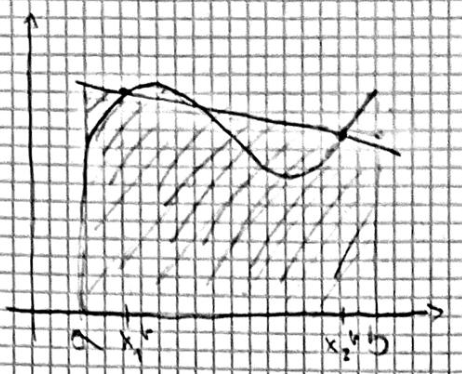
\includegraphics[width=0.5\textwidth]{images/gaussian_quad1.png}
\end{center}
The error:
$$
I(f)-\tilde{I}_G(f)=\frac{1}{4320}(b-a)^5f^{(4)}(\rho)
$$
The Gaussian rule with two nodes ($J=2$) provides same degree of exactness and results of Simpson rule with one less node (Simpson used $J=3$ nodes).

If we introduce intervals (composite Gaussian case), we will get discontinuous approximate function.

\begin{LARGE}
    $$
    \tilde{I}_G^c(f)=\frac{H}{2}
    \sum_{i=1}^H
    \left[
        f(x_1^{G,i})+
        f(x_2^{G,i})
    \right]
    $$
\end{LARGE}
\begin{center}
    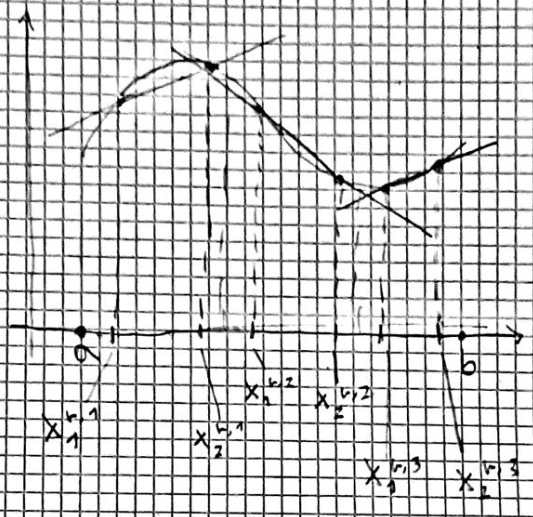
\includegraphics[width=0.5\textwidth]{images/gaussian_quad2.png}
\end{center}
The error:
$$
I(f)-\tilde{I}_G(f)=\frac{(b-a)}{4320}H^4f^{(4)}(\nu)
$$
And in conclusion:
$$
oa=4\qquad de=3
$$
In general for degree $J$ we have $2J$ unknowns and $de=2J-1$

\subsection{Numerical Differentiation}
The goal is approximate derivative of a function \textbf{at a certain single value}:
$$
f'(\overline{x})\qquad f\in C^1\left([a,b]\right)\qquad\overline{x}\in [a,b]
$$
Starting from the definition of derivative:
$$
f'(\overline{x})=\lim_{h\rightarrow 0}
\frac{
    f(\overline{x}+h)-f(\overline{x})
}{h}
$$
\subsubsection{Forward and backward finite difference}
\begin{itemize}
    \item \textbf{Forward finite difference}
    $$
    f'(\overline{x})\cong \delta_+f(\overline{x})=
    \frac{
        f(\overline{x}+h)-f(\overline{x})
    }{h}
    $$
    For $h$ closer to 0, this difference will be sharper. If we build the characteristic polynomial:
    $$
    \Pi_1f\qquad(\overline{x}, f(\overline{x}))\qquad(\overline{x}+h,f(\overline{x}+h))
    $$
    And derive it, we get exactly the forward finite difference:
    $$
    \Pi_1f(x)=f(\overline{x})
    \underlabel{
        \phi_{\overline{x}}(x)
    }{$\frac{x-\overline{x}-h}{\overline{x}-\overline{x}-h}$}
    +
    f(\overline{x}+h)
    \underlabel{
        \phi_{\overline{x}+h}(x)
    }{$\frac{x-\overline{x}}{\overline{x}+h-\overline{x}}$}=
    f(\overline{x})\frac{x-\overline{x}-h}{h}+f(\overline{x}+h)\frac{x-\overline{x}}{h}
    $$
    $$
    (\Pi_1f(x))'=-f(\overline{x})\frac{1}{h}+f(\overline{x}-h)\frac{1}{h}=
    \frac{f(\overline{x}+h)-f(\overline{x})}{h}=\delta_+f(\overline{x})
    $$
    $$
    \left(\Pi_1,f\right)'=\delta_+f(\overline{x})
    $$
    To compute the error we use the Taylor expansion:
    $$
    f(\overline{x}+h)=f(\overline{x})+hf'(\overline{x})+\frac{h^2}{2}f''(\alpha)\qquad\alpha\in [\overline{x},\overline{x}+h]\qquad f\in C^2([a,b])
    $$
    Divide everything by $h$:
    $$
    f'(\overline{x})+
    \underlabel{
        \frac{f(\overline{x})}{h}-\frac{f(\overline{x}+h)}{h}
    }{$-\delta_+f(\overline{x})$}
    =
    -\frac{h}{2}f'(\alpha)
    $$
    So:
    $$
    -\frac{h}{2}f''(\alpha)=f'(\overline{x})-\delta_+f(\overline{x})
    $$
    This scheme is a first order scheme ($h$ has degree 1).
    \item \textbf{Backward finite difference}
    $$
    f'(\overline{x})\cong \delta_-f(\overline{x})=
    \frac{
        f(\overline{x})-f(\overline{x}-h)
    }{h}
    $$
    In terms of accuracy, this scheme is equivalent fo the forward finite difference, still a first order scheme. Using the Taylor expansion to compute the error:
    $$
    f(\overline{x}-h)=f(\overline{x})-hf'(\overline{x})+\frac{h^2}{2}f''(\beta)\qquad\beta\in [\overline{x}-h,\overline{x}]\qquad f\in C^2([a,b])
    $$
    Divide everything by $h$, make computations, we will get:
    $$
    \frac{h}{2}f''(\beta)=f'(\overline{x})-\delta_-f(\overline{x})
    $$
    The same error with an inverted sign.
\end{itemize}

\subsubsection{Centered finite difference}
How to generate a scheme with higher accuracy, e.g. of second order? We can "combine the point before and the point after":
$$
f'(\overline{x})=\lim_{h\rightarrow 0}\frac{
    f(\overline{x}+h)-f(\overline{x}-h)
}{2h}
$$
And:
$$
f'(\overline{x})\simeq \delta f(\overline{x})=\frac{
    f(\overline{x}+h)-f(\overline{x}-h)
}{2h}
$$
\textbf{Centered finite difference}, for the error we considerate two Taylor expansions and we demand $f\in C^3([a,b])$:
$$
\begin{cases}
    f(\overline{x}+h)=f(\overline{x})+
    hf'(\overline{x})+
    \frac{h^2}{2}f''(\overline{x})+
    \frac{h^3}{6}f^{(3)}(\gamma)
    \qquad \gamma\in[\overline{x},\overline{x}+h]\\
    \\
    f(\overline{x}-h)=f(\overline{x})-
    hf'(\overline{x})+
    \frac{h^2}{2}f''(\overline{x})-
    \frac{h^3}{6}f^{(3)}(\rho)
    \qquad \rho\in[\overline{x}-h,\overline{x}]\\
\end{cases}
$$
Subtract the two expansions, we will get:
$$
f(\overline{x}+h)-f(\overline{x}-h)=2hf''(\overline{x})+\frac{h^3}{6}\left[
    f^{(3)}(\gamma)+f^{(3)}(\rho)
\right]
$$
Divide by $2h$ and making the computations we get:
$$
f'(\overline{x})-\delta f(\overline{x})=
-\frac{h^2}{12}\left[
    f^{(3)}(\gamma)+f^{(3)}(\rho)
\right]
$$
This last scheme is the best one, but we might have to use the forward or backward scheme when $\overline{x}$ is one of the endpoints:
\begin{center}
    
\includegraphics[width=0.5\textwidth]{images/numdif_endpoints.png}
\end{center}